% 
% Annual Cognitive Science Conference
% Sample LaTeX Paper -- Proceedings Format
% 

% Original : Ashwin Ram (ashwin@cc.gatech.edu)       04/01/1994
% Modified : Johanna Moore (jmoore@cs.pitt.edu)      03/17/1995
% Modified : David Noelle (noelle@ucsd.edu)          03/15/1996
% Modified : Pat Langley (langley@cs.stanford.edu)   01/26/1997
% Latex2e corrections by Ramin Charles Nakisa        01/28/1997 
% Modified : Tina Eliassi-Rad (eliassi@cs.wisc.edu)  01/31/1998
% Modified : Trisha Yannuzzi (trisha@ircs.upenn.edu) 12/28/1999 (in process)
% Modified : Mary Ellen Foster (M.E.Foster@ed.ac.uk) 12/11/2000
% Modified : Ken Forbus                              01/23/2004
% Modified : Eli M. Silk (esilk@pitt.edu)            05/24/2005
% Modified : Niels Taatgen (taatgen@cmu.edu)         10/24/2006
% Modified : David Noelle (dnoelle@ucmerced.edu)     11/19/2014
% Modified : Roger Levy (rplevy@mit.edu)     12/31/2018



%% Change "letterpaper" in the following line to "a4paper" if you must.

\documentclass[10pt,letterpaper]{article}

\usepackage{cogsci}
\usepackage{pslatex}
\usepackage{apacite}
\usepackage{float} % Roger Levy added this and changed figure/table
                   % placement to [H] for conformity to Word template,
                   % though floating tables and figures to top is
                   % still generally recommended!
                   
%\cogscifinalcopy % Uncomment this line for the final submission 


%\usepackage[none]{hyphenat} % Sometimes it can be useful to turn off
%hyphenation for purposes such as spell checking of the resulting
%PDF.  Uncomment this block to turn off hyphenation.

\usepackage{graphicx}
\usepackage{amsmath}
\usepackage{xcolor}

\newcommand{\tableref}[1]{Table~\ref{#1}}
\newcommand{\figref}[1]{Figure~\ref{#1}}
\newcommand{\expref}[1]{Experiment~#1}

%\setlength\titlebox{4.5cm}
% You can expand the titlebox if you need extra space
% to show all the authors. Please do not make the titlebox
% smaller than 4.5cm (the original size).
%%If you do, we reserve the right to require you to change it back in
%%the camera-ready version, which could interfere with the timely
%%appearance of your paper in the Proceedings.

\definecolor{Red}{RGB}{180,20,140}
\newcommand{\jd}[1]{\textcolor{Red}{\textbf{[jd: #1]}}} 

\title{Replicating eye-tracking research using incremental decision tasks and web-based libraries} 
 
\author{{\large \bf Judith Degen (jdegen@stanford.edu)} \\
  Department of Psychology, 1202 W. Johnson Street \\
  Madison, WI 53706 USA
  \AND {\large \bf Leyla Kursat (lkursat@stanford.edu)} \\
  Department of Educational Psychology, 1025 W. Johnson Street \\
  Madison, WI 53706 USA}


\begin{document}

\maketitle


\begin{abstract}

\jd{write}

\textbf{Keywords:} 
psycholinguistics; experimental pragmatics;  scalar implicature; linking functions; visual world; eye-tracking
\end{abstract}


\section{Introduction}

A key method of scientific investigation in cognitive science is experimental investigation. Experimental data has informed cognitive theory-building for centuries. A key ingredient for using data to test hypotheses generated from theories is the assumption one makes as a researcher about how theoretical notions map onto empirical measurements: the \emph{linking assumption}. Indeed, empirical measurement, and the data resulting from it, are only useful and informative if the assumed linking assumption is (sufficiently) clear and justified. We argue that both clarity and justification are currently lacking for linking assumptions made for \emph{visual world eye-tracking}, a widely used experimental method in psycholinguistic research. We highlight the role that visual world eye-tracking has played in the burgeoning field of experimental pragmatics, which suffers particularly acutely from a lack of clear and justified linking assumptions. We then test an often implicitly assumed linking assumption in referential tasks: that \emph{the proportion of looks to a referent in a time window reflects participants' degree of belief that the referent is the intended target in that time window}. To do so, we compare eye movement data against explicit beliefs collected in an incremental decision task. We make use of a previously collected eye movement dataset on scalar implicature processing \cite<\expref{3}>{sun2020}, \jd{which we also replicate in a web-based eye-tracking paradigm using \texttt{webgazer.js}  (\expref{1})}. We collect explicit beliefs to test against the original and replicated eye movement data in \expref{2}. 

\section{Linking assumptions for visual world eye-tracking}

\begin{itemize}
	\item VWP \cite<VWP,>{tanenhaus1995,SedivyEtAl1999:Achieving-Incremental-Semantic-, LeffelXiangKennedy2016:Imprecision-is-Pragmatic-} \jd{others like sun and breheny, kurumada, ryskin, degen, many others?} 
	\item linking functions eye-tracking: \citeNP{SalverdaTanenhaus2017:The-Visual-World-Paradigm, tanenhaus2000eye, AllopennaEtAl1998:Tracking-the-Time-,magnuson2019fixations} -- allopenna et al used gating task; mention
	\item linking functions in xprag (especially tvjt): \cite{Jasbi2019, WaldonDegen2020, franke2014typical, savinelli2018, franke2016link, scholler2017semantic, tessler2019language}
	\item incremental decision task: \cite{AllopennaEtAl1998:Tracking-the-Time-,QingLD2018, KreissDegen2020}
	\item spell out the link, give it a name?
\end{itemize}



\section{Sun \& Breheny (2020) -- the original experiment}

We replicate \expref{3} of \citeA{sun2020}. 

\begin{figure}[H]
\centering
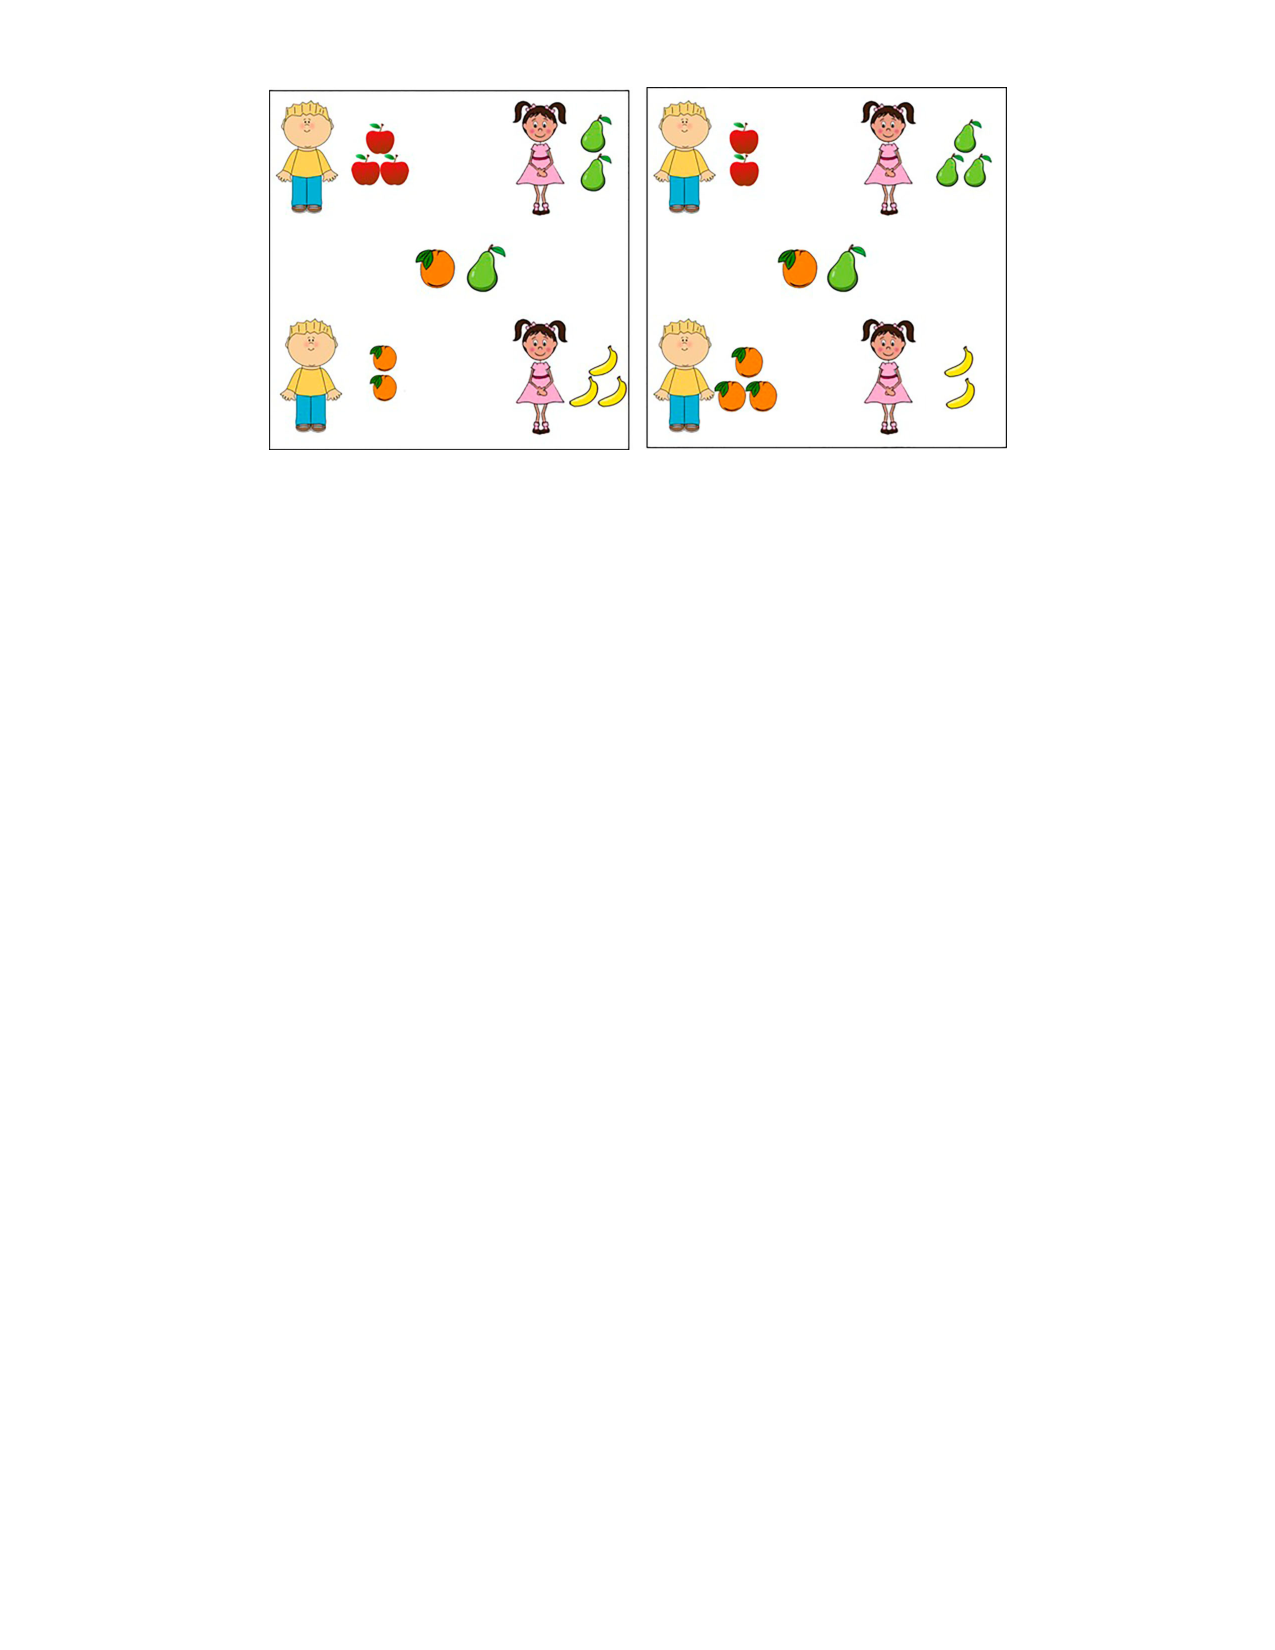
\includegraphics[width=\columnwidth]{images/display}
\caption{Example display from \expref{3} of \citeA{sun2020}. The left image (big \emph{all}/ small  \emph{some}) was paired with  \emph{Click on the boy that has all/three of Susan's apples} or  \emph{Click on the girl that has some/two of Susan's pears}. The right image (small  \emph{all}/ big  \emph{some}) was paired with  \emph{Click on the boy that has all/two of Susan's apples} or  \emph{Click on the girl that has some/three of Susan's pears}.} 
\label{fig:display}
\end{figure}

\begin{figure}
\centering
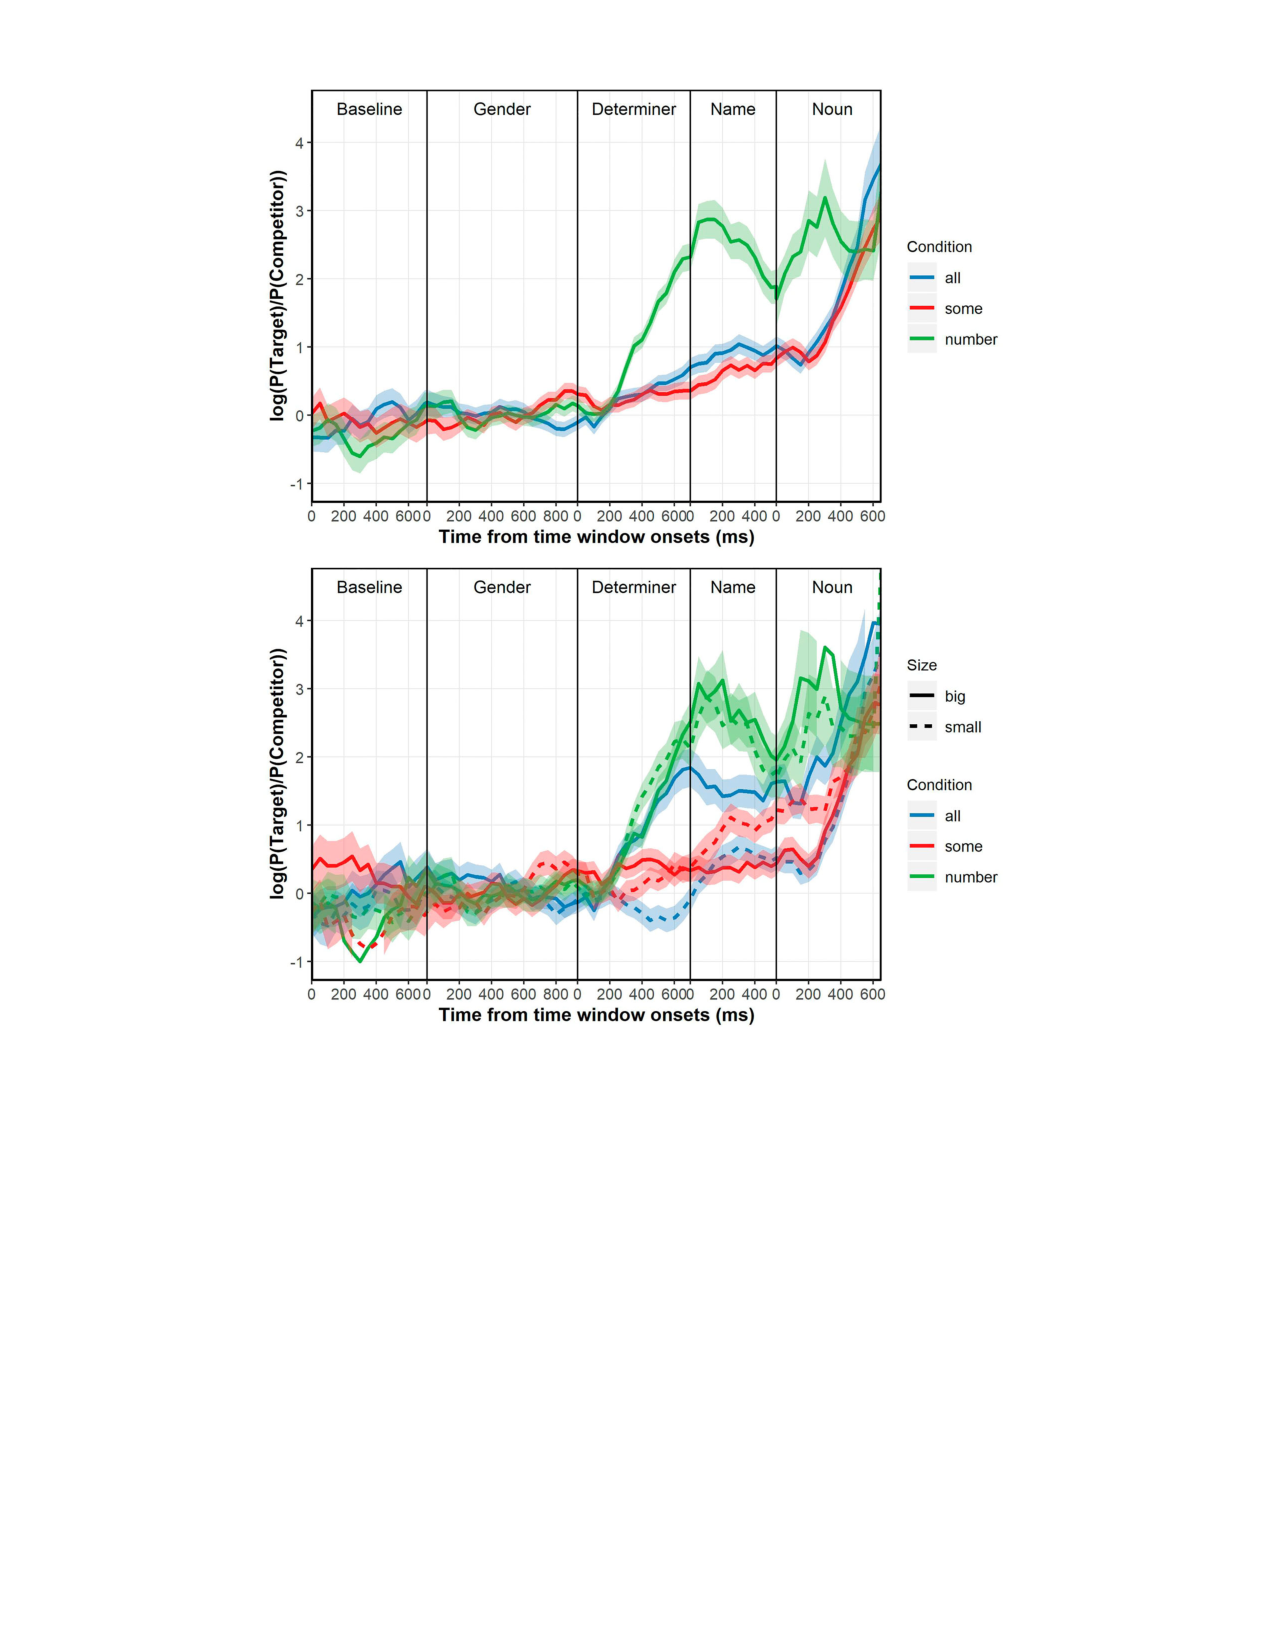
\includegraphics[width=\columnwidth]{images/results-original}
\caption{Eye movement results for \expref{3} of \citeA{sun2020}. Shown are target preference scores from instruction onset to instruction offset. Top: target preference scores by determiner type. Bottom: target preference scores by determiner type and target set size. Transparent ribbons indicate standard error.} 
\label{fig:results-original}
\end{figure}


\section{Exp.~1: replicating Sun \& Breheny (2020) using web-based eye-tracking}

\subsection{Methods}

\textbf{Participants, materials, procedure.}

\subsection{Results}

\section{Exp.~2: replicating Sun \& Breheny (2020) using an incremental decision task}

\subsection{Methods}

\textbf{Participants, materials, procedure.}

\subsection{Results}

\figref{fig:results-idt} shows target advantage scores for each time window, analogous to \figref{fig:results-original} from \citeA{sun2020}.

\textbf{Data analysis}. \citeA{sun2020} fit separate regression models to the baseline, gender, determiner, name, and noun windows. We collapsed the name window into the determiner window because the name does not add information. We thus fit mixed-effects logistic regression models to the baseline, gender, determiner, and noun window,\footnote{In fact, fitting models to the noun window was impossible because participants, with very few exceptions, always chose the target. That is, there was no variance to speak of that a model could be estimated to explain.} predicting target over competitor choices from fixed effects of quantifier (reference level: ``number"), centered size (higher value: ``big"), by-item and by-subject random intercepts, and random by-subject slopes for condition and size. No effects reached significance in the baseline, gender, and noun window, as expected. In the determiner window, the window of interest, there were main effects of condition, such that target selections were less likely in both the \emph{some} ($\beta$=-2.90, $SE$=0.36, $p<$.0001) and \emph{all} ($\beta$=-2.92, $SE$=0.36, $p<$.0001) conditions, compared to the number condition. There was no main effect of size, consistent with the visual result that target selections in the number condition are not modulated by  target set size ($\beta$=-0.09, $SE$=0.26, $p<$.73). However, we did observe interactions between quantifier and size, such that small sets led to more target selections for \emph{some} ($\beta$=0.59, $SE$=0.28, $p<$.05) but to fewer target selections for \emph{all} ($\beta$=-1.27, $SE$=0.29, $p<$.0001), compared to number terms. \jd{also report target preference score analysis?}

%(Intercept)          3.77254    0.39655   9.513  < 2e-16 ***
%conditionall        -2.92409    0.36359  -8.042 8.81e-16 *** 		replicates
%conditionsome       -2.90211    0.36217  -8.013 1.12e-15 ***		replicates
%csize               -0.09207    0.26069  -0.353   0.7239    			does not replicate -- they found main effect (more looks to big set and steeper increase)
%conditionall:csize  -1.27305    0.28523  -4.463 8.08e-06 ***		replicates
%conditionsome:csize  0.59465    0.27945   2.128   0.0333 *  		does not replicate , they found null effect (but perhaps in name window? they don't report this specifically)

\begin{figure}[H]
\centering
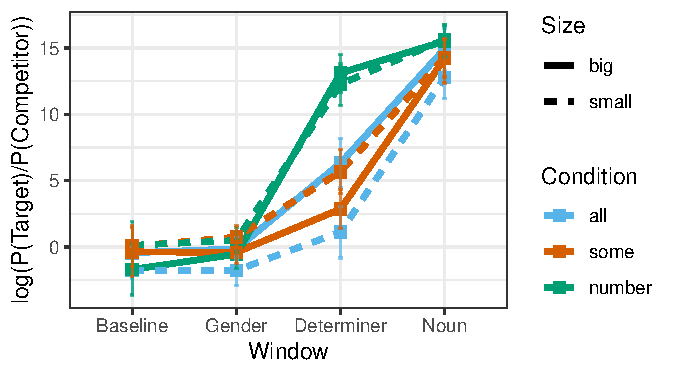
\includegraphics[width=\columnwidth]{../../analysis/SunBreheny/1_incremental/main/graphs/results-idt}
\caption{Proportions of target and competitor selections in Exp.~2 by quantifier and set size.} 
\label{fig:results-idt}
\end{figure}

\textbf{Comparison with \citeA{sun2020}: replication analysis}. These results constitute a partial replication of  \citeA{sun2020}, though we will argue that in in fact constitutes a near-exact replication. Most of their effects reported in the determiner window replicated, with two exceptions: we did not observe a main effect of set size, while they did; and we observed an interaction of size and determiner such that small \emph{some} led to greater target selections than big \emph{some}. These differences are not as big as they may seem: in our dataset, the lack of set size main effect can be explained by the interactions with determiner: while size makes no difference at all for number (the determiner predictor reference level), it has the opposite effect for \emph{all} compared to \emph{some}. A similar tendency can be observed in  \citeA{sun2020}'s results when taking into account the joint determiner and name windows. In fact,  \citeA{sun2020} report the absence of a main effect for size in the name window, and instead an interaction between size and determiner. While they do not report the same post hoc analyses, visual inspection of \figref{fig:results-original} suggests that the interaction in the name window is indeed the result of set size having the opposite effect for \emph{all} compared to \emph{some}. Thus, when taking into account their results from both the determiner and name window, which we collapsed into one, the results are qualitatively identical. The different results reported by  \citeA{sun2020} in the two time windows are presumably the result of certain information taking longer to be integrated, something which the incremental decision task by its offline nature cannot capture.

\textbf{Comparison with \citeA{sun2020}: linking function analysis}. The overall correlation between proportion of selections and proportions of looks, where proportions were calculated separately by region of interest (target, competitor, distractors), time window (baseline, gender, determiner$+$name, noun), determiner (\emph{all, some}, number), and set size (big, small), was high ($r(70) = .69$). At the individual

%Correlation between proportion of target selections in determiner window and target looks in determiner\+name window: Pearson's $r=.99$. Competitor: $r=.86$. Distractors: $r=.93$.

\jd{CONTINUE HERE DESCRIBING LINKING FUNCTION RESULTS}

\begin{figure}[H]
\centering
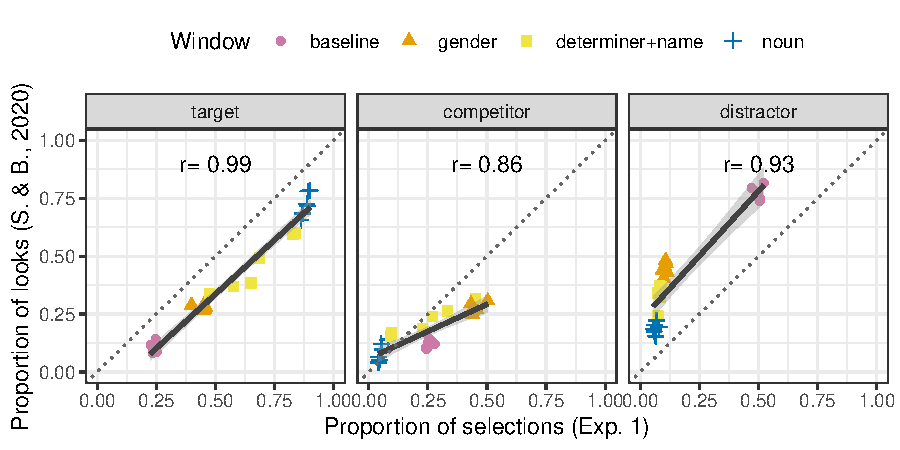
\includegraphics[width=\columnwidth]{../../analysis/SunBreheny/1_incremental/main/graphs/correlations}
\caption{Proportions of looks in \citeA{sun2020} against proportions of selections in \expref{1}. Facets indicate regions, colors indicate time window.} 
\label{fig:results-correlations}
\end{figure}

\begin{figure}[H]
\centering
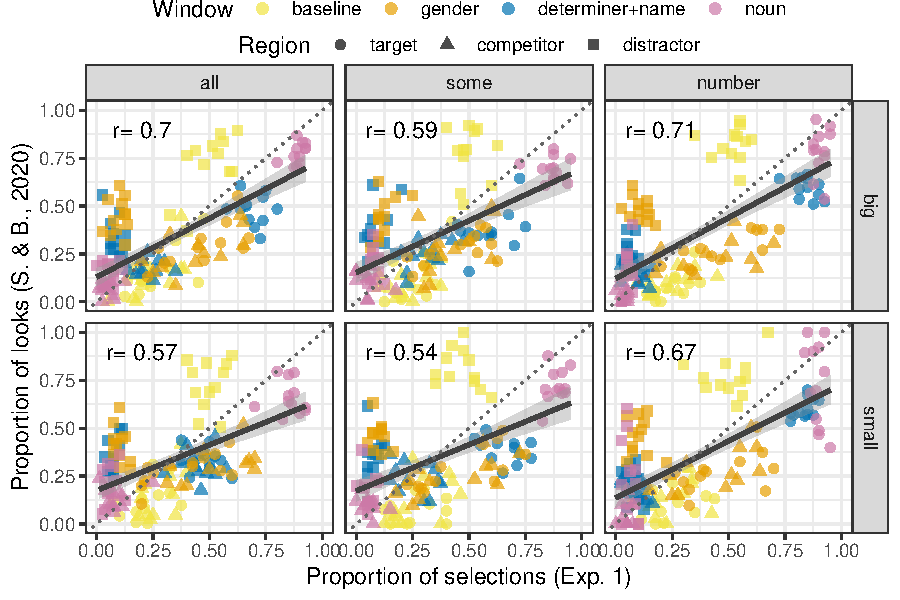
\includegraphics[width=\columnwidth]{../../analysis/SunBreheny/1_incremental/main/graphs/correlations-bycondition}
\caption{Proportions of looks in \citeA{sun2020} against proportions of selections in \expref{1}. Facets indicate regions, colors indicate time window.} 
\label{fig:results-correlations}
\end{figure}

\section{General discussion}


%\begin{table}[H]
%\begin{center} 
%\caption{Sample table title.} 
%\label{sample-table} 
%\vskip 0.12in
%\begin{tabular}{ll} 
%\hline
%Error type    &  Example \\
%\hline
%Take smaller        &   63 - 44 = 21 \\
%Always borrow~~~~   &   96 - 42 = 34 \\
%0 - N = N           &   70 - 47 = 37 \\
%0 - N = 0           &   70 - 47 = 30 \\
%\hline
%\end{tabular} 
%\end{center} 
%\end{table}


%\begin{figure}[H]
%\begin{center}
%\fbox{CoGNiTiVe ScIeNcE}
%\end{center}
%\caption{This is a figure.} 
%\label{sample-figure}
%\end{figure}


%\section{Acknowledgments}
%
%Madigan, Daisy; chao sun and richard breheny for generously sharing materials, data


\bibliographystyle{apacite}

\setlength{\bibleftmargin}{.125in}
\setlength{\bibindent}{-\bibleftmargin}

\bibliography{sunbrehenyreplication}


\end{document}
